\documentclass{beamer}

\usepackage[utf8]{inputenc}
\usepackage[spanish]{babel}
\usepackage{amsmath}
\usepackage[nosetup]{evan}
\usetheme{Goddard}
\hypersetup{colorlinks,allcolors=.,urlcolor=magenta}
\usepackage[table]{xcolor} % Para definir colores en tablas
\usepackage{graphicx} % Para redimensionar la tabla

\title{Investigación de Operaciones I}
\subtitle{Unidad 1: Elementos de Programación Lineal}
\author{Ricardo Jesús Largaespada Fernández}
\institute{Ingeniería de Sistemas, DACTIC, UNI}
\date{20 de Agosto, 2024}

\begin{document}

\frame{\titlepage}

\begin{frame}
\frametitle{Agenda}
\tableofcontents
\end{frame}

% ¿Qué es la Modelación?
\section{Importancia de la Modelación}
\subsection{Conceptos Básicos}
\begin{frame}
    \frametitle{¿Qué es la Modelación?}
    \begin{itemize}
        \item Proceso de transformar un problema del mundo real en un modelo matemático.
        \item Simplificación de la complejidad del problema para enfocarse en los elementos clave.
    \end{itemize}
    \begin{figure}
        \centering
        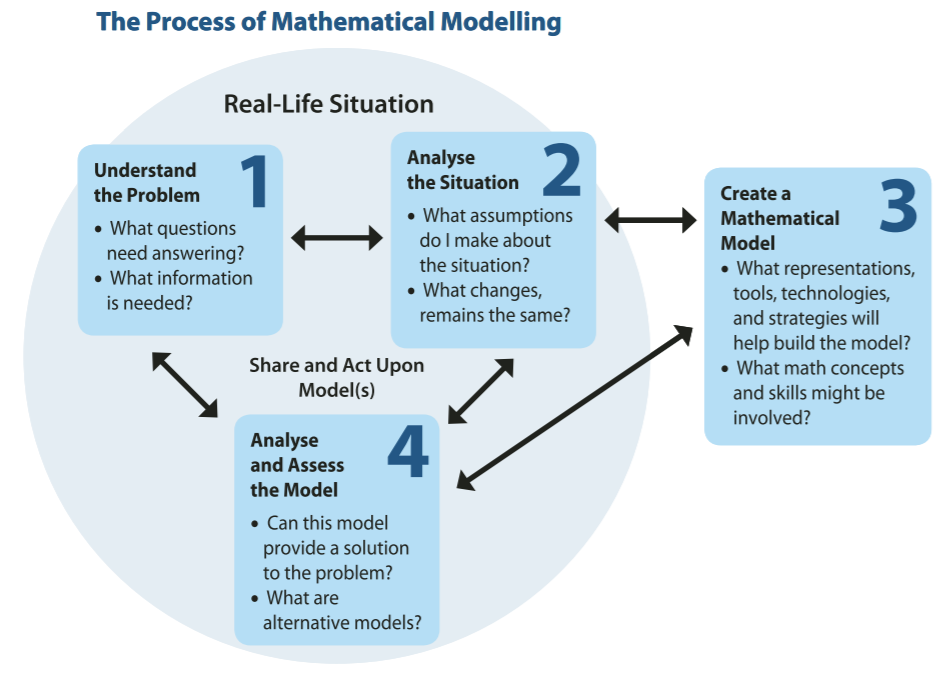
\includegraphics[width=0.5\textwidth]{images/mathematical_modelling.png} % Inserta un diagrama de ejemplo si lo tienes
    \end{figure}
\end{frame}

% Conceptos Básicos
\begin{frame}
    \frametitle{1.2.1 Conceptos Básicos}
    \begin{itemize}
        \item \textbf{Variables de Decisión:} Representan las opciones o decisiones que se pueden tomar.
        \item \textbf{Función Objetivo:} Expresión matemática que se desea maximizar o minimizar.
        \item \textbf{Restricciones:} Limitaciones que deben cumplirse en el modelo.
    \end{itemize}
    \begin{table}[]
        \centering
        \begin{tabular}{|c|c|}
            \hline
            \textbf{Concepto} & \textbf{Ejemplo} \\ \hline
            Variables de Decisión & \(x_{ij}\) \\ \hline
            Función Objetivo & Minimizar \(Z = \sum C_{ij} x_{ij}\) \\ \hline
            Restricciones & Capacidad de almacenes \\ \hline
        \end{tabular}
    \end{table}
\end{frame}

% Ejemplo Básico de Programación Lineal
\begin{frame}
    \frametitle{Ejemplo Básico de Programación Lineal}
    \textbf{Problema:} Minimizar los costos de transporte desde 2 almacenes hasta 3 tiendas.
    \begin{itemize}
        \item \textbf{Variables de Decisión:} \(x_{ij}\) (cantidad enviada de almacén \(i\) a tienda \(j\)).
        \item \textbf{Función Objetivo:} Minimizar \(Z = \sum C_{ij} x_{ij}\).
        \item \textbf{Restricciones:} Capacidad de los almacenes, demanda de las tiendas.
    \end{itemize}
    \begin{figure}
        \centering
        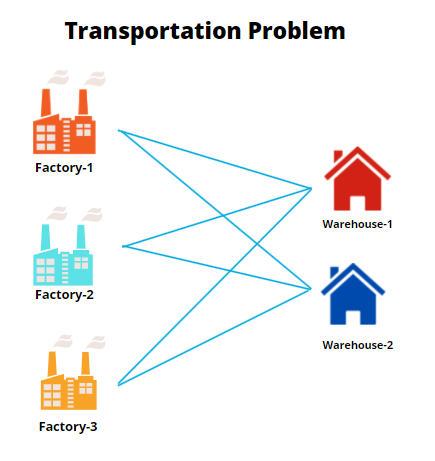
\includegraphics[width=0.5\textwidth]{images/transportation_problem.png} % Inserta un diagrama si lo tienes
    \end{figure}
\end{frame}

% Metodología General de la Modelación
\subsection{Metodología General de la Modelación}
\begin{frame}
    \frametitle{1.2.2 Metodología General de la Modelación}
    \begin{enumerate}
        \item \textbf{Definir el problema:} Identificación del objetivo y restricciones.
        \item \textbf{Formular el modelo:} Crear ecuaciones que representen el problema.
        \item \textbf{Resolver el modelo:} Encontrar la mejor solución matemática.
        \item \textbf{Validar el modelo:} Comparar con la realidad para asegurarse de su precisión.
        \item \textbf{Implementar la solución:} Aplicar la solución obtenida en la práctica.
    \end{enumerate}
\end{frame}

% Importancia de la Modelación
\begin{frame}
    \frametitle{¿Por qué es Importante la Modelación?}
    \begin{itemize}
        \item \textbf{Tomar Decisiones Informadas:} Evaluación de opciones.
        \item \textbf{Analizar Escenarios:} Evaluación de diferentes situaciones y sus impactos.
        \item \textbf{Optimización de Recursos:} Uso eficiente de los recursos disponibles.
    \end{itemize}
\end{frame}

% Ejemplos Prácticos en IO
\begin{frame}
    \frametitle{Ejemplos Prácticos en Investigación de Operaciones}
    \begin{itemize}
        \item \textbf{Optimización de la Cadena de Suministro:} Minimización de costos en la distribución de productos.
        \item \textbf{Asignación de Recursos:} Asignación de tareas a empleados.
        \item \textbf{Programación de Producción:} Maximizar la producción con recursos limitados.
    \end{itemize}
\end{frame}

% Conclusión y Preguntas
\begin{frame}
    \frametitle{Conclusión y Discusión}
    \begin{itemize}
        \item Resumen de los conceptos de modelación y metodología.
        \item Importancia de la modelación en la toma de decisiones.
        \item \textbf{Pregunta:} ¿Cómo aplicarías la modelación en tu área de estudio o trabajo?
    \end{itemize}
\end{frame}

%Tarea
\begin{frame}{Asignación}
    
\end{frame}
\end{document}
